\documentclass[../main.tex]{subfiles}
\begin{document}
\lecture{3}{07.02}{}
\section{Определение интеграла Римана. Существование интегрируемых функций. Необратимое условие}

\noindent $a<b$. Рассмотрим $[a,b]$. 
\begin{minipage}{0.5\textwidth}
    \begin{flushright}
        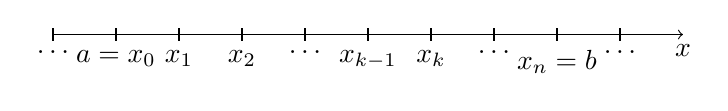
\begin{tikzpicture}[scale=0.8]
            % Draw the x-axis
            \draw[->] (-1,0) -- (9,0) node[anchor=north] {$x$};

            % Draw the points on the x-axis
            \foreach \x/\label in {-1/\dots, 0/a=x_0, 1/x_1, 2/x_2, 3/\dots, 4/x_{k-1}, 5/x_k, 6/\dots, 7/x_n=b, 8/\dots} {
                \draw (\x,0.1) -- (\x,-0.1) node[anchor=north] {$\label$};
            }
        \end{tikzpicture}
    \end{flushright}
\end{minipage}

T = \{$a=x_{0}<x_{1}<x_{2}<\dots<x_{k-1}<x_{k}<\dots<x_{n}=b$\} - разбиение отрезка [a,b]  
Рассмотрим $\Delta x_{k}=x_{k}-x_{k-1},k=1,2,3,\dots,n(k=\overline{1,n})$\\ 
$\delta_{T}\underset{1\leqslant k \leqslant n}{=} max(\Delta x_{k})$- характеристика разбиения. \\ 
$\xi_{k} \in [x_{k-1},x_{k}],k=\overline{1,n},\qquad \Xi=\{\xi_{k}\}_{k=1}^{n} $
\vspace{0.5cm}
        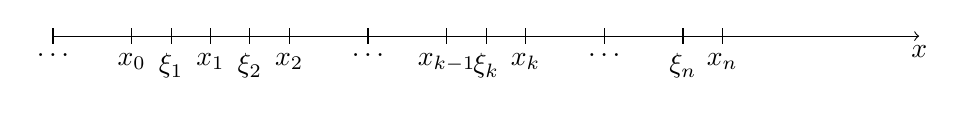
\begin{tikzpicture}[scale=1]
            % Draw the x-axis
            \draw[->] (-1,0) -- (10,0) node[anchor=north] {$x$};

            % Draw the points on the x-axis
            \foreach \x/\label in {-1/\dots, 0/x_0, 0.5/\xi_1, 1/x_1, 1.5/\xi_2, 2/x_2, 3/\dots, 4/x_{k-1}, 4.5/\xi_k, 5/x_k, 6/\dots, 7/\xi_n, 7.5/x_n, } {
                \draw (\x,0.1) -- (\x,-0.1) node[anchor=north] {$\label$};
            }
        \end{tikzpicture}

\noindent Пусть $f(x)$ определена на $[a,b]$. Рассмотрим $\displaystyle \sigma_{T}(f,\Xi)=\sum_{k=1}^{n} f(\xi_{k})\Delta x_{k}$ - интегральная сумма

\begin{definition}
    Говорят, что $\exists \lim\limits_{\delta_{T}\to 0} \sigma_{T}(f,\Xi), $ если $\exists I:\forall \varepsilon >0 \exists \delta>0: \forall T,\delta_{T}<\delta,\forall \Xi \implies |\sigma_{T}(f,\Xi)-I|<\varepsilon$
\end{definition}
! Свойства пределов переносятся.
\begin{definition}
    $f(x) $ называется интегрируемой(по Риману) на $[a,b],$ если $\exists \lim\limits_{\delta_{T}\to 0}\sigma_{T}(f,\Xi).$ Величина этого предела ($I=\lim\limits_{\delta_{T}\to 0} \sigma_{T}(f,\Xi) $) называется определенным интегралом функции $f(x)$ на $(a,b)$ (интегралом Римана))\\ 
    Обозначение: $\displaystyle \int\limits_{a}^{b}f(x)dx=I$
\end{definition}

\noindent Примеры:

а) $\displaystyle f(x)\equiv C- const \text{ на } [a,b]; \forall T=\{a=x_{0}<x_{1}<\dots<x_{n}=b\},\forall \Xi=\{\xi_{k}\}_{k=1}^{n};\\ \sigma_{T}(f,\Xi)=\sum_{k=1}^{n} f(\xi_{k})\Delta x_{k}
=\sum_{k=1}^{n} c \Delta x_{k}=c \sum_{k=1}^{n} \Delta x_{k}=c((x_{1}-x_{0})+(x_{2}-x_{1})+\dots+(x_{n}-x_{n-1})=c(x_{n}-x_{0})=\\ c(b-a) \underset{\delta_{T}\to 0}{\to}\quad c(b-a);\implies \exists \lim\limits_{\delta_{T}\to 0} \sigma_{T}(f,\Xi)=c(b-a).\implies f(x) - \text{интегрируема на } [a,b],\text{ причем } \int _{a}^{b}cdx=c(b-a)\implies$ интегрируемые функции существуют.
\newpage
б) $\chi(x)=\begin{cases}
    1, x- \text{рац.} \\  
    0, x- \text{иррац.}
\end{cases},x\in[a,b]\text{ (функция Дирихле)}\\
\text{Предположим,что }\displaystyle \exists \int\limits_{a}^{b}\chi(x)dx=I,\text{ т.е } \forall \varepsilon>0 \exists \delta>0: \forall T,\delta_{T}<\delta,\forall \Xi\implies |\sigma_{T}(\chi,\Xi)-I|<\varepsilon \\
\text{Возьмем }\Xi_{1}=\{\xi_{k}^{(1)}\}_{k=1}^{n} -\text{набор рац. точек }\qquad \sigma^{(1)}=\sigma_{T}(\chi,\Xi_{1})=\sum_{k=1}^{n}\underbrace{\chi(\xi_{k}^{(1)})}_{=1}\Delta x_{k}=b-a\\ 
\text{Возьмем } \Xi_{2}=\{\xi_{k}^{2}\}_{k=1}^{n}-\text{набор иррац. точек }\qquad \sigma^{(2)}=\sigma_{T}(\chi,\Xi_{2})=\sum_{k=1}^{n}\underbrace{\chi(\xi_{k}^{(2)})}_{=0}\Delta x_{k}=0\\ 
b-a=|\sigma^{(1)}-\sigma^{(2)}|=|\sigma^{(1)}-I-\sigma^{(2)}+I|\leqslant \underbrace{|\sigma^{(1)}-I|}_{<\varepsilon}+\underbrace{|\sigma^{(2)}-I|}_{<\varepsilon}<\varepsilon+\varepsilon=b-a-\text{противоречие}\implies \chi(x) \text{ не является интегрируемой на }[a,b]$
\begin{theorem}[Необходимое условие интегрируемости]
    $f(x)$-интегрируема на $[a,b]\implies$ $f(x)-$ ограничена на $[a,b]$
\end{theorem}
\begin{proof}
    От противного. Предположим,что $f(x)$ не является ограниченной на $[a,b]$, но при этом $\displaystyle \exists \int _{a}^{b} f(x)dx=I,\text{ т.е }$ $\forall \varepsilon >0 \exists \delta>0:\forall T,\delta_{T}<\delta, \forall \Xi\implies|\sigma_{T}(f,\Xi)-I|<\varepsilon.$\\
    Берем $\varepsilon=1\implies \exists \delta>0: \forall T,\delta_{T}<\delta,\forall \Xi \implies|\sigma_{T}(F,\Xi)-I|<1$\\
    Берем $\forall T=\{a=x_{0}<\dots<x_{k-1}<x_{k}<\dots<x_{n}=b\};$\\
    Строим $\Xi=\{\xi\}_{k=1}^{n}$
    $f(x)$ неограничена на $[a,b]\implies\exists k: f(x) $ неограничена на $[x_{k-1},x_{k}],$\\
    $\Xi: \xi_{1},\xi_{2},\dots,\xi_{k-1},\xi_{k+1},\dots,\xi_{n}-$ произвольные.\\
    Берем такое $\xi_{k}:|f(\xi_{k})|>\frac{1+|I|+|f(\xi_{1})|\Delta x_{1}+|f(\xi_{2})|\Delta x_{2} +\dots+|f(\xi_{k-1})|\Delta x_{k-1}+\dots+|f(\xi_{n})|\Delta x_{n}}{\Delta x_{k}}|$\\
    $|\sigma_{T}(f,\Xi)-I|\geqslant |\sigma_{T}(f,\Xi)|-|I|=|f(\xi_{1})\Delta x_{1}+\dots+ f(\xi_{k-1})\Delta x_{k-1}+f(\xi_{k})\Delta x_{k}+f(\xi_{k+1})\Delta x_{k+1}+\dots+f(\xi_{n})\Delta x_{n}|\allowbreak-|I|=|f(\xi_{k})\Delta x_{k}-(-f(\xi_{1})\Delta x_{1}-\dots-f(\xi_{k-1})\Delta x_{k-1}-f(\xi_{k+1})\Delta x_{k+1}-\dots-f(\xi_{n})\Delta x_{n})|-|I|\geqslant$
    \\$\geqslant |f(\xi_{k})|\Delta x_{k}-|f(\xi_{1})|\Delta x_{1}-\dots-|f(\xi_{k-1})|\Delta x_{k-1}-|f(\xi_{k+1})|\Delta x_{k+1}-\dots-|f(\xi_{n})|\Delta x_{n}-|I|>| = \varepsilon \implies \text{ противоречие}$ 
\end{proof}

\section{Суммы Дарбу и их свойства. Связь сумм Дарбу с интегральной суммой }
Пусть $f(x)$ ограничена на $\displaystyle [a,b].\quad T=\{a=x_{0}<\dots<x_{n}=b\}. $
$\begin{aligned}M_{k}\underset{x_{k-1}\leqslant x\leqslant x_{k}}{=}\sup{(f(x))};\\ m_{k}\underset{x_{k-1}\leqslant x\leqslant x_{k}}{=}\inf{(f(x))}.\end{aligned}$\\$ S_{T}(f) =\sum_{k=1}^{n}M_{k}\Delta x_{k}-\text{верхняя сумма Дарбу.}\\ $
$ s_{T}(f)=\sum_{k=1}^{n}m_{k}\Delta x_{k}-\text{нижняя сумма Дарбу}$\\
Эти суммы не обязаны быть интегральными суммами, т.к точные грани не всегда достигаются. \\
$ \forall \Xi=\{ \xi_{k}\}_{k=1}^{n}\implies m_{k}\leqslant f(\xi_{k})\leqslant M_{k}. \qquad s_{T}(f)\leqslant \sigma_{T}(f,\Xi)\leqslant S_{T}(f)$
\begin{definition}
    $T_{1}=\{a=x_{0}^{(1)}<x_{1}^{(1)}<\dots<x_{n}^{(1)}=b\}\qquad
    T_{2}=\{a=x_{0}^{(2)}<x_{1}^{(2)}<\dots<x_{m}^{(2)}=b\}.\\
    T_{2} \text{ называется последующим к } T_{1},\text{ если } x_{k}^{(1)}\in T_{2} \forall k=\overline{0,n}.\text {Обозначение } T_{2} \succ T_{1}
    $
\end{definition}
\vspace{1cm}
\begin{theorem}
    Если $T_{1} \succ T_{2}\implies 
        \begin{aligned}
            1) & \quad S_{T_{1}}(f)\leqslant S_{T_{2}}(f) \\
            2) & \quad s_{T_{1}}(f)\geqslant s_{T_{2}}(f)
        \end{aligned}$
\end{theorem}
\begin{proof}
    1) Пусть у $T_{1}$ ровно  на 1 точку больше, т.е $\begin{aligned} T_{2}=\{a=x_{0}<x_{1}<\dots<x_{k-1}<x_{k}<\dots<x_{n}<b\}.\\
T_{1}=\{a=x_{0}<x_{1}<\dots<x_{k-1}<\tilde{x}<x_{K}<\dots<x_{n}=b\}.\end{aligned}$\\ 
    $M_{k}\underset{x_{k-1}\leqslant x\leqslant x_{k}}{=}\sup f(x),\quad M_{k}'\underset{x_{k-1}\leqslant x\leqslant \tilde{x}}{=}\sup{f(x)}\leqslant M_{k},\quad M_{k}''\underset{\tilde{x}\leqslant x\leqslant x_{k}}{=}\sup{f(x)}\leqslant M_{k}$\\ 
    Рассмотрим $ S_{T_{2}}(f)-S_{T_{1}}(f)=M_{k}\Delta x_{k}-M_{k}'(\tilde{x}- x_{k-1})-M_{k}''(x_{k}-\tilde{x})=M_{k}(x_{k}-x_{k-1})-M_{k}'(\tilde{x}-x_{k-1})-M_{k}''(x_{k}-\tilde{x})=M_{k}(x_{k}-\tilde{x}+\tilde{x}-x_{k-1})-M_{k}'(\tilde{x}-x_{k-1})=\underbrace{(M_{k}-M_{k}'')}_{\geqslant 0}\underbrace{(x_{k}-\tilde{x})}_{>0}+\underbrace{(M_{k}-M_{k}')}_{\geqslant 0}\underbrace{(\tilde{x}-x_{k-1})}_{>0}\geqslant 0\implies S_{T_{2}}(f)\geqslant S_{T_{1}}(f).$ Если у $T_{1}$ более, чем на одну точку больше, то делаем аналогично нужное число раз.
 \end{proof}

\begin{theorem}
    $\forall T_{1},T_{2}\implies s_{T_{1}}(f)\leqslant S_{T_{2}}(f)$
\end{theorem}
\begin{proof}
    Рассмотрим $T_{3}=T_{1} \cup T_{2} \implies \begin{cases}
        T_{3}\succ T_{1} \\
        T_{3}\succ T_{2}
    \end{cases}\implies s_{T_{1}}(f)\underset{\text{Т2.2}}{\leqslant} s_{T_{3}}(f)\leqslant S_{T_{3}}(f)\underset{\text{Т2.2}}{\leqslant} S_{T_{2}}(f)$
\end{proof}
\begin{theorem}
    $ \forall T, \forall \varepsilon>0 \exists \Xi_{1},\exists \Xi_{2}:\begin{cases}
        0\leqslant S_{T}(f)-\sigma_{T}(f,\Xi_{1})<\varepsilon \\ 
        0\leqslant \sigma_{T}(f,\Xi_{2})-s_{T}(f)<\varepsilon
    \end{cases}$
\end{theorem}
\begin{proof}
    Берем $ \forall T =\{a=x_{0}<x_{1}<\dots<x_{k-1}<x_{k}<\dots<x_{n}=b\}. \qquad \begin{aligned}M_{k}\underset{x_{k-1}\leqslant x\leqslant x_{k}}{=}\sup{(f(x))},\\m_{k}\underset{x_{k-1}\leqslant x\leqslant x_{k}}{=}\inf{(f(x))} \end{aligned}
    \implies \forall \varepsilon > 0 \begin{aligned}\exists \xi_{k}^{(1)}\in [x_{k-1},x_{k}]: 0\leqslant M_{k}-f(\xi_{k}^{(1)})<\frac{\varepsilon}{b-a}\\ 
    \exists \xi_{k}^{(2)}\in [x_{k-1},x_{k}]:0\leqslant f(\xi_{k}^{(2)})-m_{k}<\frac{\varepsilon}{b-a}\end{aligned}$
    $\left| \Delta x_{k} \text{ и } \sum_{k=1}^{n} \right.\implies \begin{aligned}
        0\leqslant S_{T}(f)-\sigma_{T}(f,\Xi_{1})<\varepsilon\\
        0\leqslant \sigma_{T}(f,\Xi_{2})-s_{T}(f)<\varepsilon
    \end{aligned}$
\end{proof}
\section{Верхний и нижний интегралы Дарбу. Критерий интегрируемости}
Из теоремы 2.3 $\implies \forall T_{1},T_{2}\quad \underbrace{s_{T_{1}}(f)}_{\text{огр. сверху}}\leqslant \underbrace{S_{T_{2}}(f)}_{\text{огр. снизу}}$\\ 
Рассмотрим $\bar{I}\underset{T}{=}\inf{S_{T}(f)} -\text{ верхний интеграл Дарбу}.$
$\underbar{I}\underset{T}{=}\sup{s_{T}(f)} - \text{ нижний интеграл Дарбу}$\\ 
$ s_{T_{1}}(f)\leqslant S_{T_{2}}(f).\qquad \underbar{I}\leqslant S_{T_{2}}(f).\qquad$ \fbox{$\underbar{I}\leqslant \bar{I}$}
\begin{theorem}[Критерий интегрируемости]
    $f(x)$ интегрируема на $[a,b]\Leftrightarrow \lim\limits_{\delta_{T}\to 0}(S_{T}(f)-s_{T}(f))=0 $
\end{theorem}
\begin{proof}
    $\implies$ $f(x)$ интегрируема на $[a,b]$ $\displaystyle \implies \exists \int\limits_{a}^{b} f(x)dx=I,\text{ т.е } \forall \varepsilon>0 \exists \delta >0 : \forall T,\delta_{T}<\delta \implies|\sigma_{T}(f,\Xi)-I|<\frac{\varepsilon}{4},\text{ т.е } I-\frac{\varepsilon}{4}<\sigma_{T}(f,\Xi)<I+\frac{\varepsilon}{4} \\ 
    \text{Но } \varepsilon>0 \underset{\text{Т2.4}}{\implies} \exists \Xi_{1},\exists \Xi_{2}: \begin{aligned} 0\leqslant S_{T}(f)-\sigma_{T}(f,\Xi_{1})<\frac{\varepsilon}{4}\\ 
    0\leqslant \sigma_{T}(f,\Xi_{2})-s_{T}(f)<\frac{\varepsilon}{4} \end{aligned}\\ 
    I-\frac{\varepsilon}{2}<\sigma_{T}(f,\Xi_{2})-\frac{\varepsilon}{4}<s_{T}(f)\leqslant S_{T}(f)<\sigma_{T}(f,\Xi_{1})+\frac{\varepsilon}{4}<I +\frac{\varepsilon}{2}\\ \implies
    0\leqslant S_{T}(f)-s_{T}(f)<\varepsilon\implies\lim\limits_{\delta_{T}\to 0}(S_{T}(f)-s_{T}(f))=0 $
    \\ 
    $\impliedby \text{ Пусть } \lim\limits_{\delta_{T}\to 0}(S_{T}(f)-s_{T}(f))=0,\text{т.е } \forall \varepsilon>0 \exists \delta>0: \forall T,\delta_{T}<\delta\implies 0\leqslant S_{T}(f)-s_{T}(f)<\varepsilon$\\ 
    \noindent
    $\text{Но } s_{T}(f)\leqslant \underbar{I}\leqslant \bar{ I} \leqslant S_{T}(f)\implies 0\leqslant \bar{I}-\underbar{I}<\varepsilon\implies\bar{I}-\underbar{I}=0\implies \underbar{I}=\bar{I}.\\ \text{ Обозначим } \underbar{I}=\bar{I}=I
    \implies\left.\begin{aligned}&s_{T}(f)\leqslant I\leqslant S_{T}(f)\\ 
    &\text{Но } \forall \Xi \implies s_{T}(f)\leqslant \sigma_{T}(f,\Xi)\leqslant S_{T}(f)\end{aligned}\right\} \implies |\sigma_{T}(f,\Xi)-I|<\varepsilon \implies \exists \lim\limits_{\delta_{T}\to 0} \sigma_{T}(f,\Xi)=I\implies f(x) - \text{ интегрируема на } [a,b]$
\end{proof}
\begin{corollary}
    $f(x)$ интегрируема на $[a,b]\implies \lim\limits_{\delta_{T}\to 0}s_{T}(f)=\lim\limits_{\delta_{T}\to 0}S_{T}(f)=I (\exists \displaystyle \int _{a}^{b}f(x)dx=I)$
\end{corollary}
\vspace{0.2cm}
\begin{proof}
    $f(x)$ инт на $[a,b]$$\implies \begin{aligned}
        &1) \lim\limits_{\delta_{T}\to 0}(S_{T})(f)-s_{T}(f))=0 \\ 
        &2) \int _{a}^{b}f(x)dx=I, \forall T s_{T}(f)\leqslant I\leqslant S_{T}(f) 
    \end{aligned}$$\implies 0\leqslant S_{T}(f)-I\leqslant S_{T}(f)-s_{T}(f); 0\leqslant I-s_{T}(f)\leqslant \underbrace{S_{T}(f)-s_{T}(f)}_{\underbrace{\to 0}_{\delta_{T} \to 0}}
    \implies\left. \begin{aligned}
        \lim\limits_{\delta_{T}\to 0}(S_{T}(f)-I)=0 \\ 
        \lim\limits_{\delta_{T}\to 0}(I-s_{T}(f))=0 
    \end{aligned}\right\} $$\implies \lim\limits_{\delta_{T}\to 0}S_{T}(f)=\lim\limits_{\delta_{T}\to 0}s_{T}(f)=I$.
\end{proof}
\end{document}